%IOE Latex Template originally
%prepared by Ramesh Bhandari 072/MSI/610
% modified by Dr. Basanta Joshi
\documentclass[12pt,a4paper,oneside]{report}
\usepackage{multirow}
\usepackage{rotating}
\usepackage{hhline}
\usepackage{graphicx}
\graphicspath{{./Graphics/}} 
\usepackage[left=1.5in, right=1in,top=1in,bottom=1in,headheight=6pt, a4paper]{geometry}
\usepackage{titling}
\usepackage{booktabs}
\usepackage{natbib}
%\usepackage{times}
\usepackage{microtype}
\usepackage{amsmath}
\usepackage{enumitem}
\usepackage[font=normalsize,labelfont=bf,tableposition=top]{caption}
\usepackage{setspace}
\usepackage[explicit]{titlesec}
\usepackage[ruled,vlined]{algorithm2e}


\linespread{1.3}
\setlength{\parskip}{6pt}
\setlength{\parindent}{0em}
\titleformat{\chapter}[display]
    {\centering\normalfont\normalsize\bfseries}{\MakeUppercase{\chaptertitlename} \thechapter}{0pt}{\normalsize #1}
\titlespacing{\chapter}{0pt}{0pt}{20pt}


\titleformat{\section}
  {\normalfont\normalsize\bfseries}{\thesection}{1em}{#1}

\titleformat{\subsection}
  {\normalfont\normalsize\bfseries}{\thesubsection}{1em}{#1}

\titleformat{\subsubsection}
  {\normalfont\normalsize\bfseries}{\thesubsubsection}{1em}{#1}

\renewcommand{\baselinestretch}{1.5}



\title{DEHRA.COM
}
\author{RAJ MAHARJAN}
\date{\today}


\renewcommand{\bibname}{REFERENCES}
\renewcommand\contentsname{TABLE OF CONTENTS}
\renewcommand{\listfigurename}{LIST OF FIGURES}





\begin{document}

\begin{titlingpage} 
\begin{normalsize}
\begin{center}

\includegraphics[width=1.5in, height=1in]{Graphics/logo.jpg}\\

\bfseries 
TRIBHUVAN UNIVERSITY\\
 INSTITUTE OF ENGINEERING\\

\textbf{SAGARMATHA ENGINEERING COLLEGE}\\
\end{center}
\vspace{0.8cm}

\begin{center}
\textbf{A PROJECT PROPOSAL ON}\\
\textbf{\thetitle} \\
\vspace{1.3cm}
\bfseries BY\\
\textbf{RODAN RAMDAM SEC074BCT035}\\
\textbf{RAJ MAHARJAN SEC074BCT032}\\
\textbf{BISHWAS DANGOL SEC074BCT011}\\
\textbf{ANU SHARMA SEC074BCT009}\\
\vspace{1.3cm}
\textls[-50]{\textbf{A PROJECT PROPOSAL SUBMITTED TO THE DEPARTMENT OF ELECTRONICS AND COMPUTER ENGINEERING IN PARTIAL FULFILLMENT OF THE REQUIREMENTS FOR THE DEGREE OF BACHELOR IN COMPUTER ENGINEERING}}\\
\vspace{1.5cm}
\bfseries \textls[-50] {DEPARTMENT OF ELECTRONICS AND COMPUTER ENGINEERING}\\
SANEPA, LALITPUR, NEPAL\\
\vspace{1.5cm}
\thedate
\end{center}
\end{normalsize}
\end{titlingpage}
%================================================================
\newpage
%==============================Abstract Page=================================================
\pagenumbering{roman}
\setcounter{page}{1}
\chapter*{ABSTRACT}
\addcontentsline{toc}{chapter}{ABSTRACT}
\thispagestyle{plain} 
A place to stay is always has been the one of the important parts of  human’s day to day life. Similarly, in the case of Nepal, according to Annual Household Survey 2016/2017 by CBS, Nepal \cite{householdsurvey} which was released in 2019, 24.7 percent of people in urban areas don’t own their own house either choosing to stay in an apartment or rent a room however from talking with various people from different places of our locality, people have problem finding rooms in the place they want and compare for the best price they can get. Applications that do exist which have tried to solve this problem seems to be missing more function which could be integrated in order to make life of people easier. Even on the context of current situation, where the world is suffering from world-wide COVID-19 pandemic the option of choosing the best option for them and contacting the house owner and renter before the room is actually rented virtually has been even more necessary with the choice of showing the actual way towards the house for a person who want to rent in order for them to come in contact with as less people as possible is more important in current scenario. Not only for current situation but even in the world when there are no more huge implications by COVID, features as such could help day-to-day people get rooms efficiently and room renters to get their preferred choice i.e. most people prefer certain types of people to rent their rooms such as students. 
\par
\textbf{Keywords:} Room Renting Nepal, Google Map API Integration, DBMS(Database Management System), Real Time Chat, MVC Approach(Model View Controller), Flutter Android Application Development, Python Backend with Flask, Object Relational Mapper Tool, ReactJs Web Application Development
%\keywords{Room Renting Nepal  \and Google Map API Integration \and DBMS(Database Management System) \and Real Time Chat \and  MVC Approach(Model View Controller \and Flutter Andriod Application Development \and Python Backend with Flask \and Object Relational Mapper \and ReactJs Web Application Development}
%=============================================================================================
\newpage

\renewcommand{\baselinestretch}{0.5}
\addcontentsline{toc}{chapter}{\contentsname}{\tableofcontents}
\newpage
\renewcommand{\baselinestretch}{1.5}
\addcontentsline{toc}{chapter}{\listfigurename}{ \listoffigures}
\newpage

\chapter*{LIST OF ABBREVIATIONS}
\addcontentsline{toc}{chapter}{LIST OF ABBREVIATIONS}

DBMS\hspace{11mm}: Database Management System\\
API\hspace{16mm}: Application Program Interface\\
SQL\hspace{15mm}: Structured Query Language\\
MVC\hspace{13.1mm}: Model View Controller\\
REST API\hspace{3mm}: RestFul Application Program Interface\\





\pagenumbering{arabic}
\chapter{INTRODUCTION}
Home has always been a place where one’s comfort zone lies. A place where people can rest from their day-to-day stress, think about something new, have time for oneself or their family. Not all people can afford to build a house hence they go to the second option of renting a room or an apartment.

\section{Background }
 People tend to rent their place which comforts them the most i.e. people tend to rent near there work place or study place.

\section{Problem Definition}
 Finding place where one has never been to is very time consuming and even when searching might not result on finding even on empty room. Even when searching online, there is no proper way of talking to the owner in a secure manner i.e. either a site just give the phone number of the owner to the public or they just send them an email and reveal their location to the public. This has a security flaw since owners personal information is out there in public.
\section{Problem Solution}
 The solution to the problem can be seen in following ways:
 \begin{itemize}
 	\item Create an application through which owner and renter can talk with each other through the application.
 	\item Owner can approve for showing of their information if they find the request legit through chatting features in the application.
 	\item Renter can book the room after both owner and renter approves after which through google maps integration, renter can use it to find the way to owners house.
 \end{itemize}
\section{Objectives}
This work is conducted in order to: 
\begin{itemize}
  \item To make it easier for average citizen to rent a room
  \item To make it easier for average house owner to rent out a room
   
\end{itemize}
\chapter{LITERATURE REVIEW}
The main idea of this project is to make renting of rooms for average citizen easier through improving several features such as adding way of having live chat, google maps integration allowing users to use the feature of following path to reach the destination, only reveling necessary data such as rent per month, location i.e. place’s name only, Image of the place, etc. other data being shared when user allows it to be shared. \\
Various renting systems such has house renting system\cite{houserent}, car renting system projects have been done one of them being from Bangladesh, house renting system being focused on entire property similar to ‘basobas.com’. Other products such as ‘rentalnepal.com’, ‘gharbazar.com’, ‘gharbheti.com’ and even in ‘hamrobazar.com’ already exist all trying to solve their own ways. All of these have solved one problem but removing some important features from previous products i.e. Some give phone numbers only, one only allows through there emailing service, one totally lacks images of the rooms posted in the site. All of these problems were the main reason this project is viable. \\
In order for this project to go on forward Web application development, Android application development and knowledge about DBMS was necessary. For all of these, React Js., Flutter, Flask and PostgreSQL were all the technology planned to be used with the help of Object Relational Mapper Tool such as SQLAlchemy. In optional technology, Node Js. is kept so that all the planned features could be integrated even if there is any problem which may occur during backend using Flask.

\chapter{METHODOLOGY}
\section{Process Model}
In this project, we opted to follow agile model\cite{agile} since we felt it was the best way of going forward learning the technology, easier way of learning together and is used during production on companies. Since in this model we can build  our application in various iterations, working application features needed later on if found important could be integrated easily. This model also promotes teamwork and allow for cross-training i.e. allows us to go on with our plan of making both web application through React Js. and Android Application through Flutter. Debugging should also be easier using this model since at the beginning small application of doing main task of booking the room could be developed then including the other parts on later iterations making it easier and helping to find out the bug on the software quicker. Documentation could also be done easily which is important since the project is to be done in such time constraint. 
\begin{figure}[ht]
	\centering
	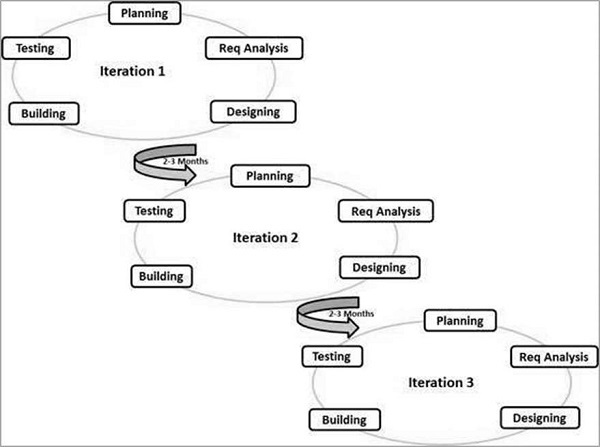
\includegraphics[width=\linewidth,height=250px]{Graphics/sdlc_agile_model.jpg}
	\caption{Agile Model\cite{agile} }
\end{figure}

\section{Tools to be used}

\subsection{Android}
Android is an Linux kernel based mobile operating system managed by Google. It is used by several smartphones and tablets. Example includes Samsung Galaxy, OnePlus, etc. \\
Unlike Apple's iOS, Android is an open source i.e. developer can modify or customize the OS for each phone. Even this is the case, application on similar android version can run on all the platform regradless of the vendor of the phone and unlike iOS, application can be deployed for testing and presenting purpose on an actual phone though any PC while iOS needs a MAC.

\subsection{Android Studio}
Android Studio is an official Integrated Development Environment(IDE) for Android, based on IntelliJ IDEA. On top of IntelliJ's powerful code editor and developer tools, Android Studio even offers more features that enhances your productivity with building Android Application.\\
Virtual android device is one of the important features which allow testing of files in different virtual android devices. Using developer mode's USB debugging mode feature.

\subsection{VSCode}
Visual Studio Code is a lightweight but powerful source code editor.  It comes with built-in support for JavaScript, TypeScript and Node.js and has a rich ecosystem of extensions for other languages (such as C++, C\#, Java, Python, PHP, Go) and runtimes (such as .NET and Unity).\\
This IDE also allow android application development though testing in users mobile through the developer mode's USB debugging mode feature.
\subsection{Flask}
Flask is an microframework made from Python. Here the word 'micro' doesn't mean that it lacks functionality but is simple in it's core but is extensible. Decisions such as which database to use is not decided by flask and decisions of flask such as it's template engine of Jinja can be changed easily. 
\subsection{React Js.}
React is a JavaScript library for building user interfaces. React has been designed from the start for gradual adoption, and you can use as little or as much React as you need.
\subsection{Flutter}
Flutter is Google’s UI toolkit for building beautiful, natively compiled applications for mobile, web, and desktop from a single codebase. In it's core, it uses dart programming language. It has features of fast development, good native performance with expressive and flexible UI.
\subsection{PostgreSQL}
PostgreSQL is a powerful, open source object-relational database system that uses and extends the SQL language combined with many features that safely store and scale the most complicated data workloads.\\
PostgreSQL has earned a strong reputation for its proven architecture, reliability, data integrity, robust feature set, extensibility, and the dedication of the open source community behind the software to consistently deliver performance and innovative solutions. PostgreSQL runs on all major operating systems, has been ACID-compliant since 2001, and has powerful add-ons such as the popular PostGIS geospatial database extender.\\
\subsection{SQLAlchemy}
SQLAlchemy is the Python SQL toolkit and Object Relational Mapper that gives application developers the full power and flexibility of SQL.\\
It provides a full suite of well known enterprise-level persistence patterns, designed for efficient and high-performing database access, adapted into a simple and Pythonic domain language.
\section{Block Diagram}
\begin{figure}[ht]
	\centering
	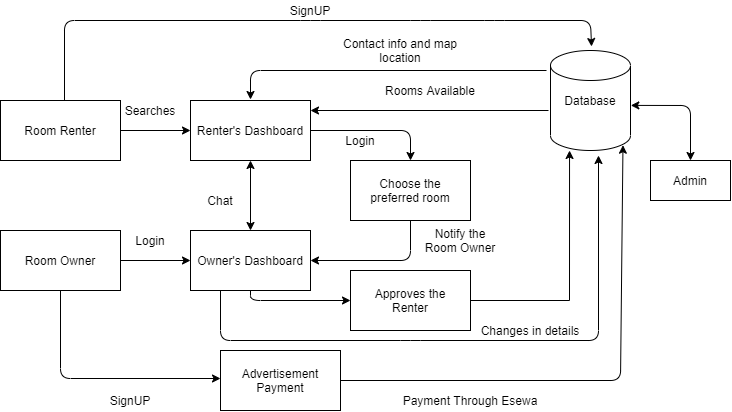
\includegraphics[width=\linewidth, height=250px]{Graphics/diagram.png}
	\caption{System Block Diagram }
\end{figure}
When room renter opens the application an interface which allows the user to check rooms available. In order to choose the room they prefer login is needed and if there is no account then room renter has to signup. After the room renter has signed in and choosen there prefered room, notification is sent to the room owner. \\
When Room Owner opens the application, owner has to signup initally and choose advertisement plan then do online payment through the application. Next time they can just login then be presented to owner's dashboard where they can update more information about their room. If renter chooses their room then they can chat with the room renter.\\
After chatting through the application, if both come to an agreement, owner can then share their number and location by approving the renter. Renter can then find the rented room through the Google Map route from the application.\\
Admin can review all the transactions and could change data in database for improvement.\\
\section{Algorithm}
\begin{algorithm}[H]
	Step1: Looks for the content \\
	Step2:\While{User Finds proper room or exits}{
	Step3: \uIf{User Logged in}{
				Goto Step6
			}
			\uElseIf{User account exists}{
				Goto Step5
			}
			\uElse{
				Goto Step4
			}
	Step4: Signup for new account\\
	Step5: Login\\
	Step6: Choose Preferred room(Notification is sent to the Room owner)\\
	Step7: Chatting with the Room owner through the application\\
	Step8: \uIf{Room Owner Agrees}{
				Recieves detail i.e. Map and contact info.
			}\uElse{
				Recieves info that the request has been denied.
			}
	}
	\caption{For Room Renter}
\end{algorithm}
This Algorithm shows how a room renter can use our application.\\
\begin{algorithm}[H]
	Step1: \uIf{User Logged in}{
				Goto Step4
			}
			\uElseIf{User account exists}{
				Goto Step3
			}
			\uElse{
				Goto Step2
			}
	Step2: Signup for new account\\
	Step3: Registers for Advertisement\\
	Step4: Login\\
	Step5: \uIf{User want to change detail}{
				Change detail
			}
	Step6: \While{No requests}{
				No requests
			}
	Step7: Chatting with the Room Renter through the application.
	Step8: \uIf{Approves}{
				Goto Step9
			}
			\uElse{
				Rejects the applicant and they get the information\\
				Goto Step6
			}
	Step9: Option of sending phone number, Location of the house through maps.
	\caption{For Room Owner}
\end{algorithm}
This Algorithm shows how a room owner can use our application.

\chapter{FEASIBILITY STUDY}
A feasibility analysis is used to determine the viability of an idea, such as ensuring a project is legally and technically feasible as well as economically justifiable. It tells us whether a project is worth the investment—in some cases, a project may not be doable. There was research done in order to check the feasibility.
\section{Technical Feasibility}
The task focused include front end in React Js. and Flutter, backend using Flask and Node js.(when needed) and DBMS using PostgreSQL, for map Google provides there Google Maps API. All of these are chosen due to there application on various stuffs like making better design to being easily extensible and main point being open source. All of these make it feasible to apply on software level. For hardware level following are the chosen:
\subsection{PC}
Computer with following features are chosen:
\begin{enumerate}[label=(\alph*)]
	\item Processor:	Intel(R) Core(TM) i5-6200U CPU @ 2.30GHz, 2401 Mhz, 2 Core(s), 4 Logical Processor(s)
	\item Physical Memory: 4.00 GB
	\item Graphics Card: AMD Radeon (TM) R5 M330
\end{enumerate}
\subsection{Android}
Flutter Supports all the application above Android Jelly Bean 4.1.x or newer but in our case Marshmellow 6.0 is used.
\section{Economic Feasibility}
Since most of the software/program/framework being used is open source it doesn't have a big effect in the total budget of the software development. One which does require initial investment is Google's Map API which depends upon features chosen but afterwards Google gives 200\$ credit per month which enough in per month basis unless there is a overload where additional payment might be necessary. \\
Only other investment is for the labour work. All of the initial investment could be recovered though the owners sharing their rooms in our application.
\section{Time Feasibility}
Since our work flow is planned through agile model, working application can be released soon and features could be added eventually. To reach our goals, a gannt chart was developed planning the estimated time for each task. Each task were given bit more time as needed so that if needed it goal could be reached easily finishing the project on time. 
\section{Operational Feasibility}
Although due to COVID-19 pandemic physical interview could not be held but still though the mediums like Facebook, interviews were conducted. Several people pointed us to the fact that there are applications which already exists and approved on the point that most of them lacks feature we planned to include and that it would help them if they were to rent a room and would use application that is easier for them.
\chapter{WORK SCHEDULE}
\begin{figure}[ht]
\centering
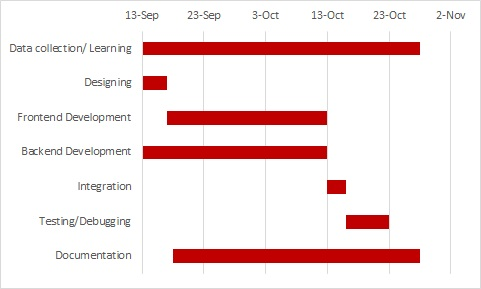
\includegraphics[width=\linewidth]{Graphics/time.JPG}
\caption{Time schedule }
\end{figure}

\begin{enumerate}[label=(\alph*)]
	\item Data Collection/Learning refers to the data being added to the database in order to make the application and learning how to apply them. Since this can go concurrently with other works being done and takes less time than others, it is taking full project time.
	\item Designing is the time for making UI/UX for frontend developement. It has been given 4 days since we are using Agile model, this could be improved on later iteration. It starts on the first day of the project.
	\item Frontend Development is the part to code the interface costumers see and act on. Since it is connected with designing part it's given 26 days giving interface development 1 month to complete. 
	\item Backend Development is the part where all of the data are stored and is needed to be kept secure. Hence, all of the 1 month is given to this task and it starts on the first day of the project. Team is divided into frontend and backend so that things could be done concurrently.
	\item Integration is the part of combining frontend and backend of the program. Several Errors might occur hence, 3 days are given for this.
	\item Testing/Debugging is the part where anyone except the development group is given the application to try and if bug is found it is patched out.
	\item Documentation is the part of writing down everything that has been done in the project hence making it easier for debugging and changing on future iterations.
\end{enumerate}
 
\chapter{EXPECTED OUTPUT}
Dehra is an multi platform application to make renting rooms easier for average citizen. The room renter can find rooms in any location s/he prefers and can contact the owner through the application which removes calls from unknown number for owner making it easier for owner to know who are interested. Although the location is given, to give map of the owner's room, owner needs to approve making it more secure for the owner and the map navigation feature helps the renter reach the destination easier. Both renter and owner can provide feedback which can be analysed to make the application better on future versions.

\newpage
\bibliographystyle{unsrt}
\bibliography{refrences/ref.bib}
\addcontentsline{toc}{chapter}{REFERENCES}

\end{document}